\documentclass[12pt,aspectratio=169]{beamer}


\usepackage{algorithm,algorithmic}

\usepackage[utf8]{inputenc}
\usepackage{booktabs}
\usepackage[opacity=0.1]{pdfcomment} % set to 0 to make annotation icons invisible
\usepackage{pdfpc}
\usepackage{arev}
\usepackage{multicol}

\usepackage{xcolor, color, colortbl}
\definecolor{dkgreen}{rgb}{0,0.5,0}
\definecolor{dkred}{rgb}{0.8,0,0}
\definecolor{dkblue}{rgb}{0,0,0.5}
\definecolor{gray}{rgb}{0.5,0.5,0.5}
\definecolor{mauve}{rgb}{0.58,0,0.82}
\definecolor{hilight}{RGB}{122,86,0}

\definecolor{LRed}{rgb}{1,.8,.8}
\definecolor{MRed}{rgb}{1,.6,.6}
\definecolor{HRed}{rgb}{1,.2,.2}

\usepackage{tikz}
\usetikzlibrary{arrows.meta,
                calc, chains,
                quotes,
                positioning,
                shapes.geometric}


\def\scalefact{0.85}
\newcommand{\cev}[1]{\reflectbox{\ensuremath{\vec{\reflectbox{\ensuremath{#1}}}}}}
\newcommand{\evalat}[2]{\left.#1\right\vert_{#2}}

\newcommand{\znode}[5][black]{\path (#3,#4) node(#2) [circle,draw,color=#1] {#5};}
\newcommand{\zunedge}[6][black]{%
\begin{scope}
	\path (#2,#3) node(this) [inner sep=0pt,triangle,draw,color=#1] {#4};
	\draw[->,color=#1] (#5) -- (this.west);
	\draw[->,color=#1] (this.east) -- (#6);
\end{scope}}
\newcommand{\zbiedge}[7][black]{%
\begin{scope}
	\path (#2,#3) node(this) [inner sep=0pt,triangle,draw,color=#1] {#4};
	\draw[->,color=#1] (#5) -- (this);
	\draw[->,color=#1] (#6) -- (this);
	\draw[->,color=#1] (this.east) -- (#7);
\end{scope}}
\newcommand{\zedge}[5][black]{\path (#3,#4) node(#2) [inner sep=0pt,triangle,draw,color=#1] {#5};}

\definecolor{blue(pigment)}{rgb}{0.2, 0.2, 0.6}
\definecolor{burgundy}{rgb}{0.5, 0.0, 0.13}


\usepackage{listings}
%% \usetheme{Goettingen}
\usefonttheme{serif}
\usepackage{times}
\setbeamertemplate{navigation symbols}{}

%\newcommand{\Grid}[2]{%
%  \def\maxX{#1}
%  \def\maxY{#2}
%  \begin{tikzpicture}
%    \draw[line width=1pt] (0,0) rectangle (\maxX,\maxY);
%    \foreach \x in {0,1,...,\maxX}{
%    \draw (\x,0) -- (\x,\maxY);
%    \draw[line width=1pt] (\maxX*0.5,0) -- (\maxX*0.5,\maxY);
%    \draw[line width=1pt,red] (\maxX*0.25,0) -- (\maxX*0.25,\maxY);
%    \draw[line width=1pt,red] (\maxX*0.75,0) -- (\maxX*0.75,\maxY);
%    }
%    %
%    \foreach \y in {0,1,...,\maxY}{
%    \draw (0,\y) -- (\maxX,\y);
%    \draw[line width=1pt] (0,\maxY*0.5) -- (\maxX,\maxY*0.5);
%    \draw[line width=1pt,red] (0,\maxY*0.25) -- (\maxX,\maxY*0.25);
%    \draw[line width=1pt,red] (0,\maxY*0.75) -- (\maxX,\maxY*0.75);
%    }
%  \end{tikzpicture}
%}

\title{Deep Learning}
\subtitle{Lecture 11: Convolutional Neural Network}
 
 
%\author[Mehrdad Maleki] % (optional, for multiple authors)
%{Mehrdad Maleki, Barak A. Pearlmutter\footnote{ Institute & Department of Computer Science
%Maynooth University, Co. Kildare, Ireland}, Jeffrey Mark Siskind}
 
%\institute[NUIM] % (optional)
%{
%  Department of Computer Science \\
%  National University of Ireland Maynooth
 
%}

\author[]{\textbf{Dr. Mehrdad Maleki}}
%\institute[]{\textsuperscript{1}Department of Computer Science\\ National University of Ireland\\ Maynooth}
 
\date{}
 
%\logo{\includegraphics[height=1.5cm]{lion-logo.png}}

\renewcommand{\Re}{\mathbb{R}}
 
\begin{document}
 
\frame{\titlepage}


\begin{frame}
\begin{center}
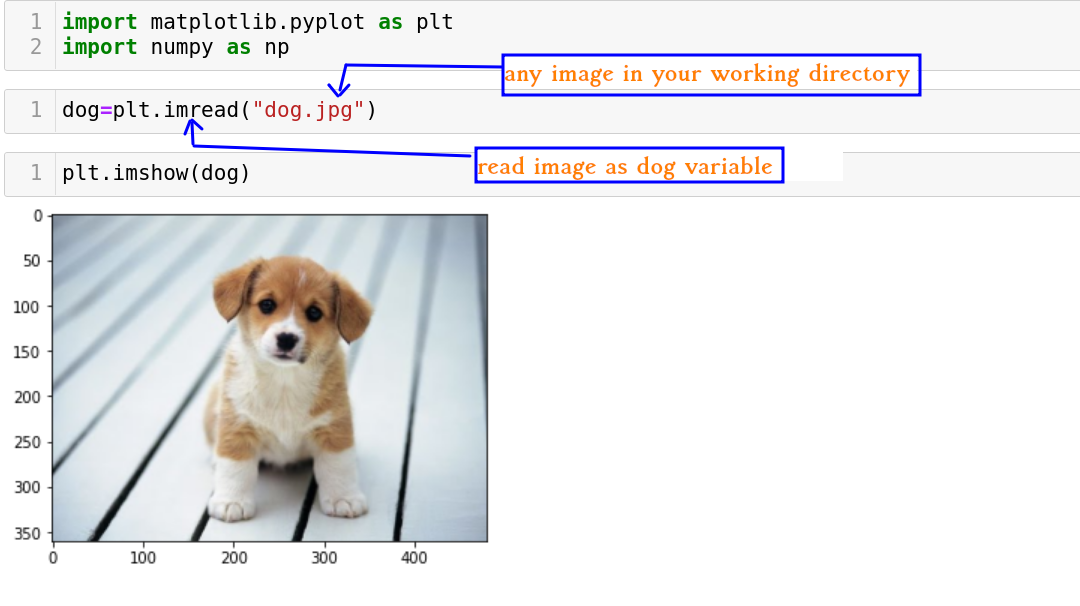
\includegraphics[scale=0.5]{dog1}
\end{center}
\end{frame}

\begin{frame}
\begin{center}
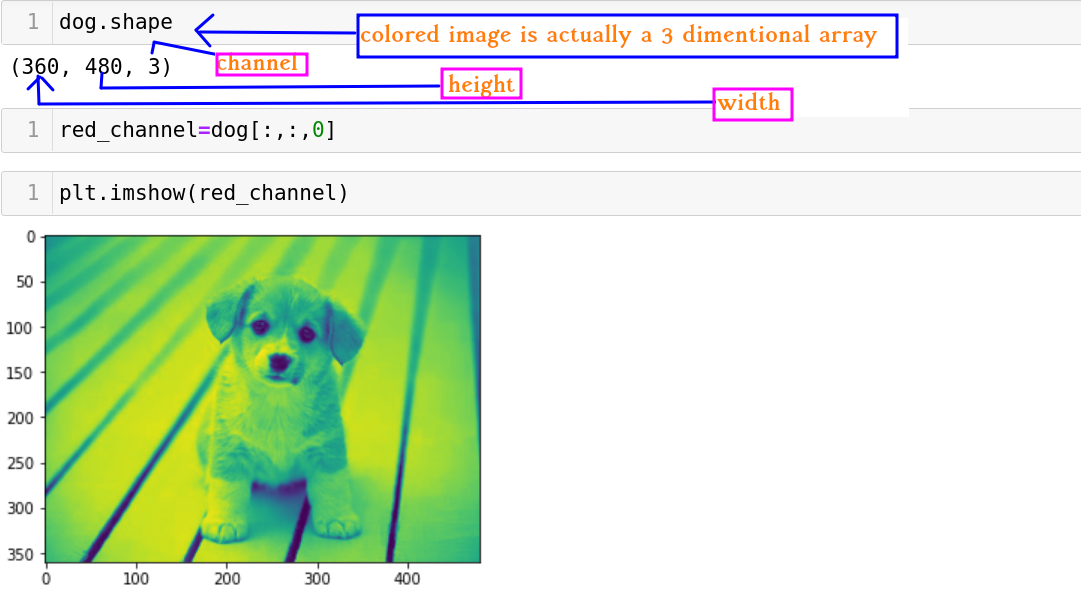
\includegraphics[scale=0.5]{dog2}
\end{center}
\end{frame}

\begin{frame}
\begin{center}
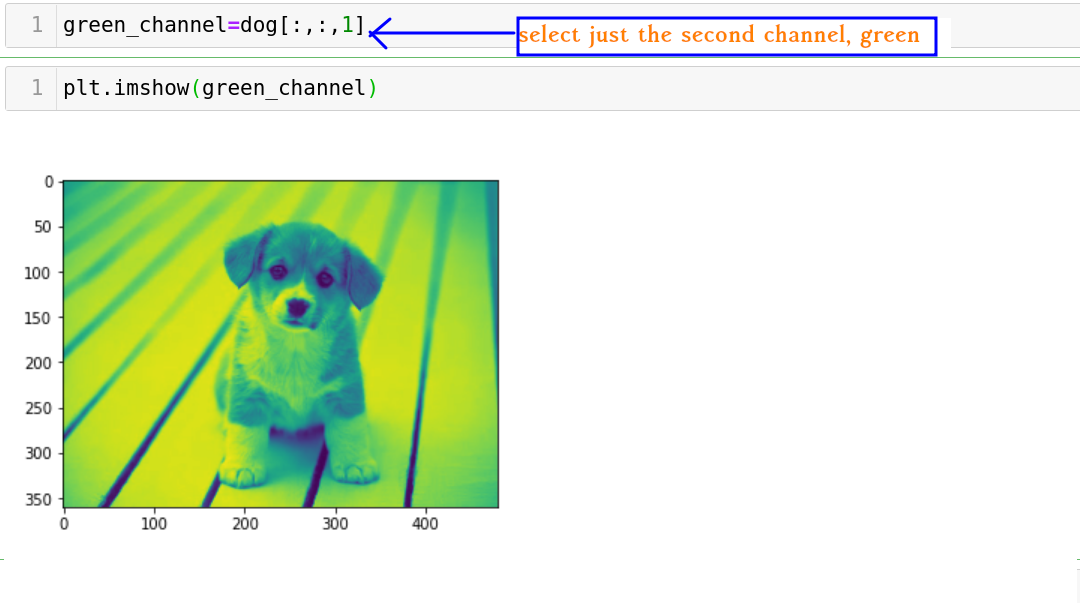
\includegraphics[scale=0.5]{dog3}
\end{center}
\end{frame}

\begin{frame}
\begin{center}
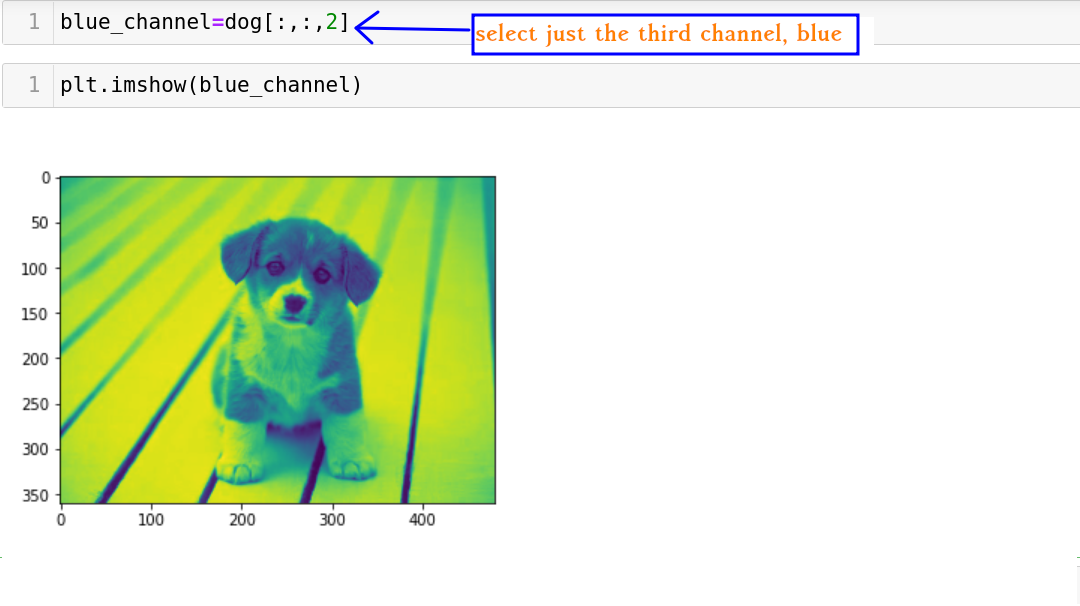
\includegraphics[scale=0.5]{dog4}
\end{center}
\end{frame}

\begin{frame}
\begin{center}
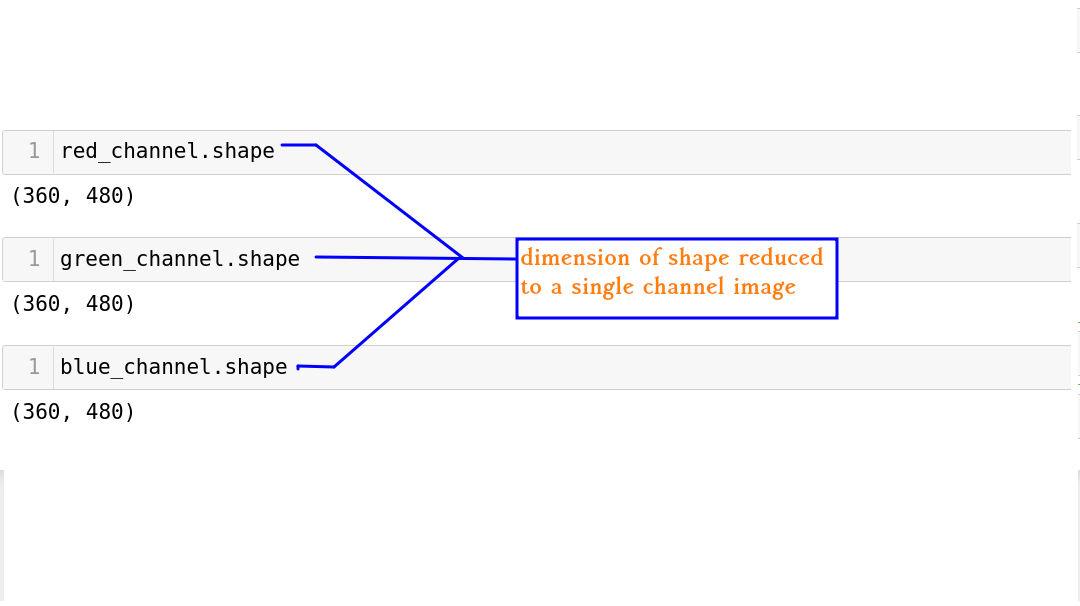
\includegraphics[scale=0.5]{dog5}
\end{center}
\end{frame}

\begin{frame}
\begin{center}
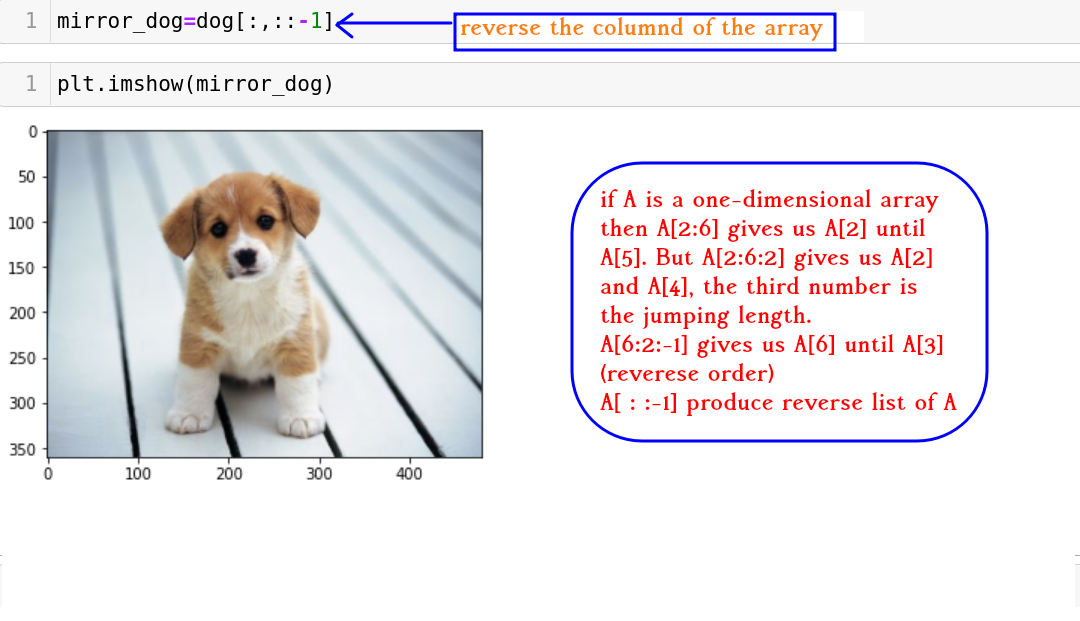
\includegraphics[scale=0.5]{dog6}
\end{center}
\end{frame}

\begin{frame}
\begin{center}
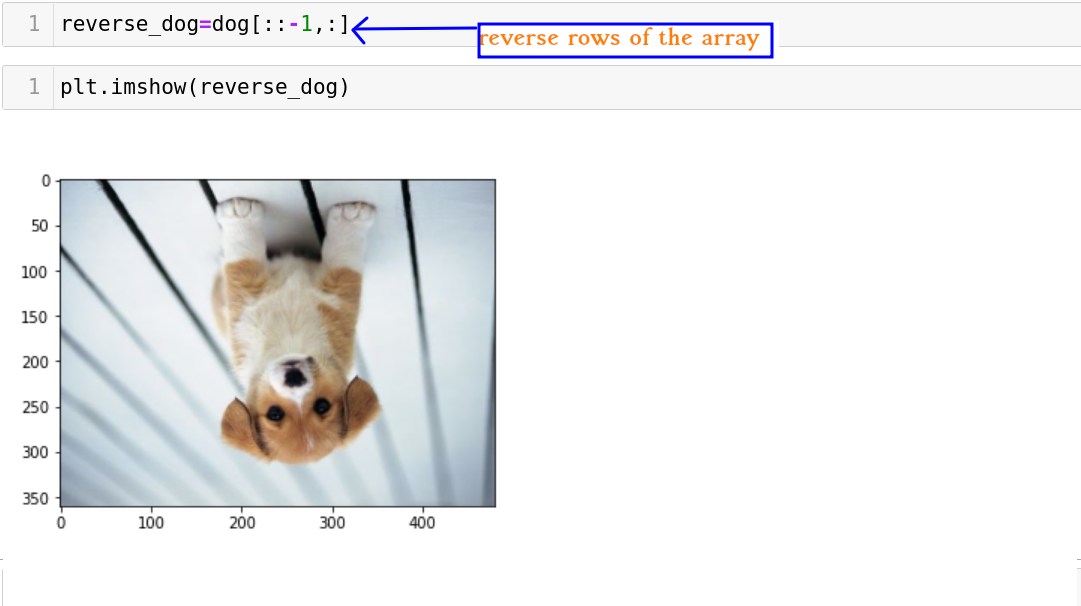
\includegraphics[scale=0.5]{dog7}
\end{center}
\end{frame}

\begin{frame}
\begin{center}
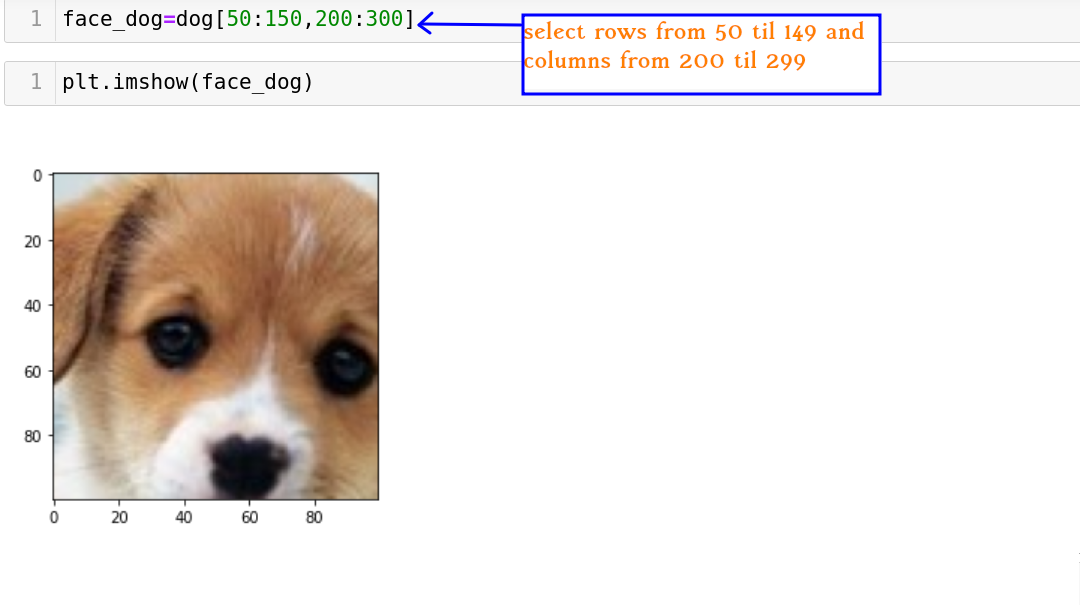
\includegraphics[scale=0.5]{dog8}
\end{center}
\end{frame}



\begin{frame}
\begin{center}
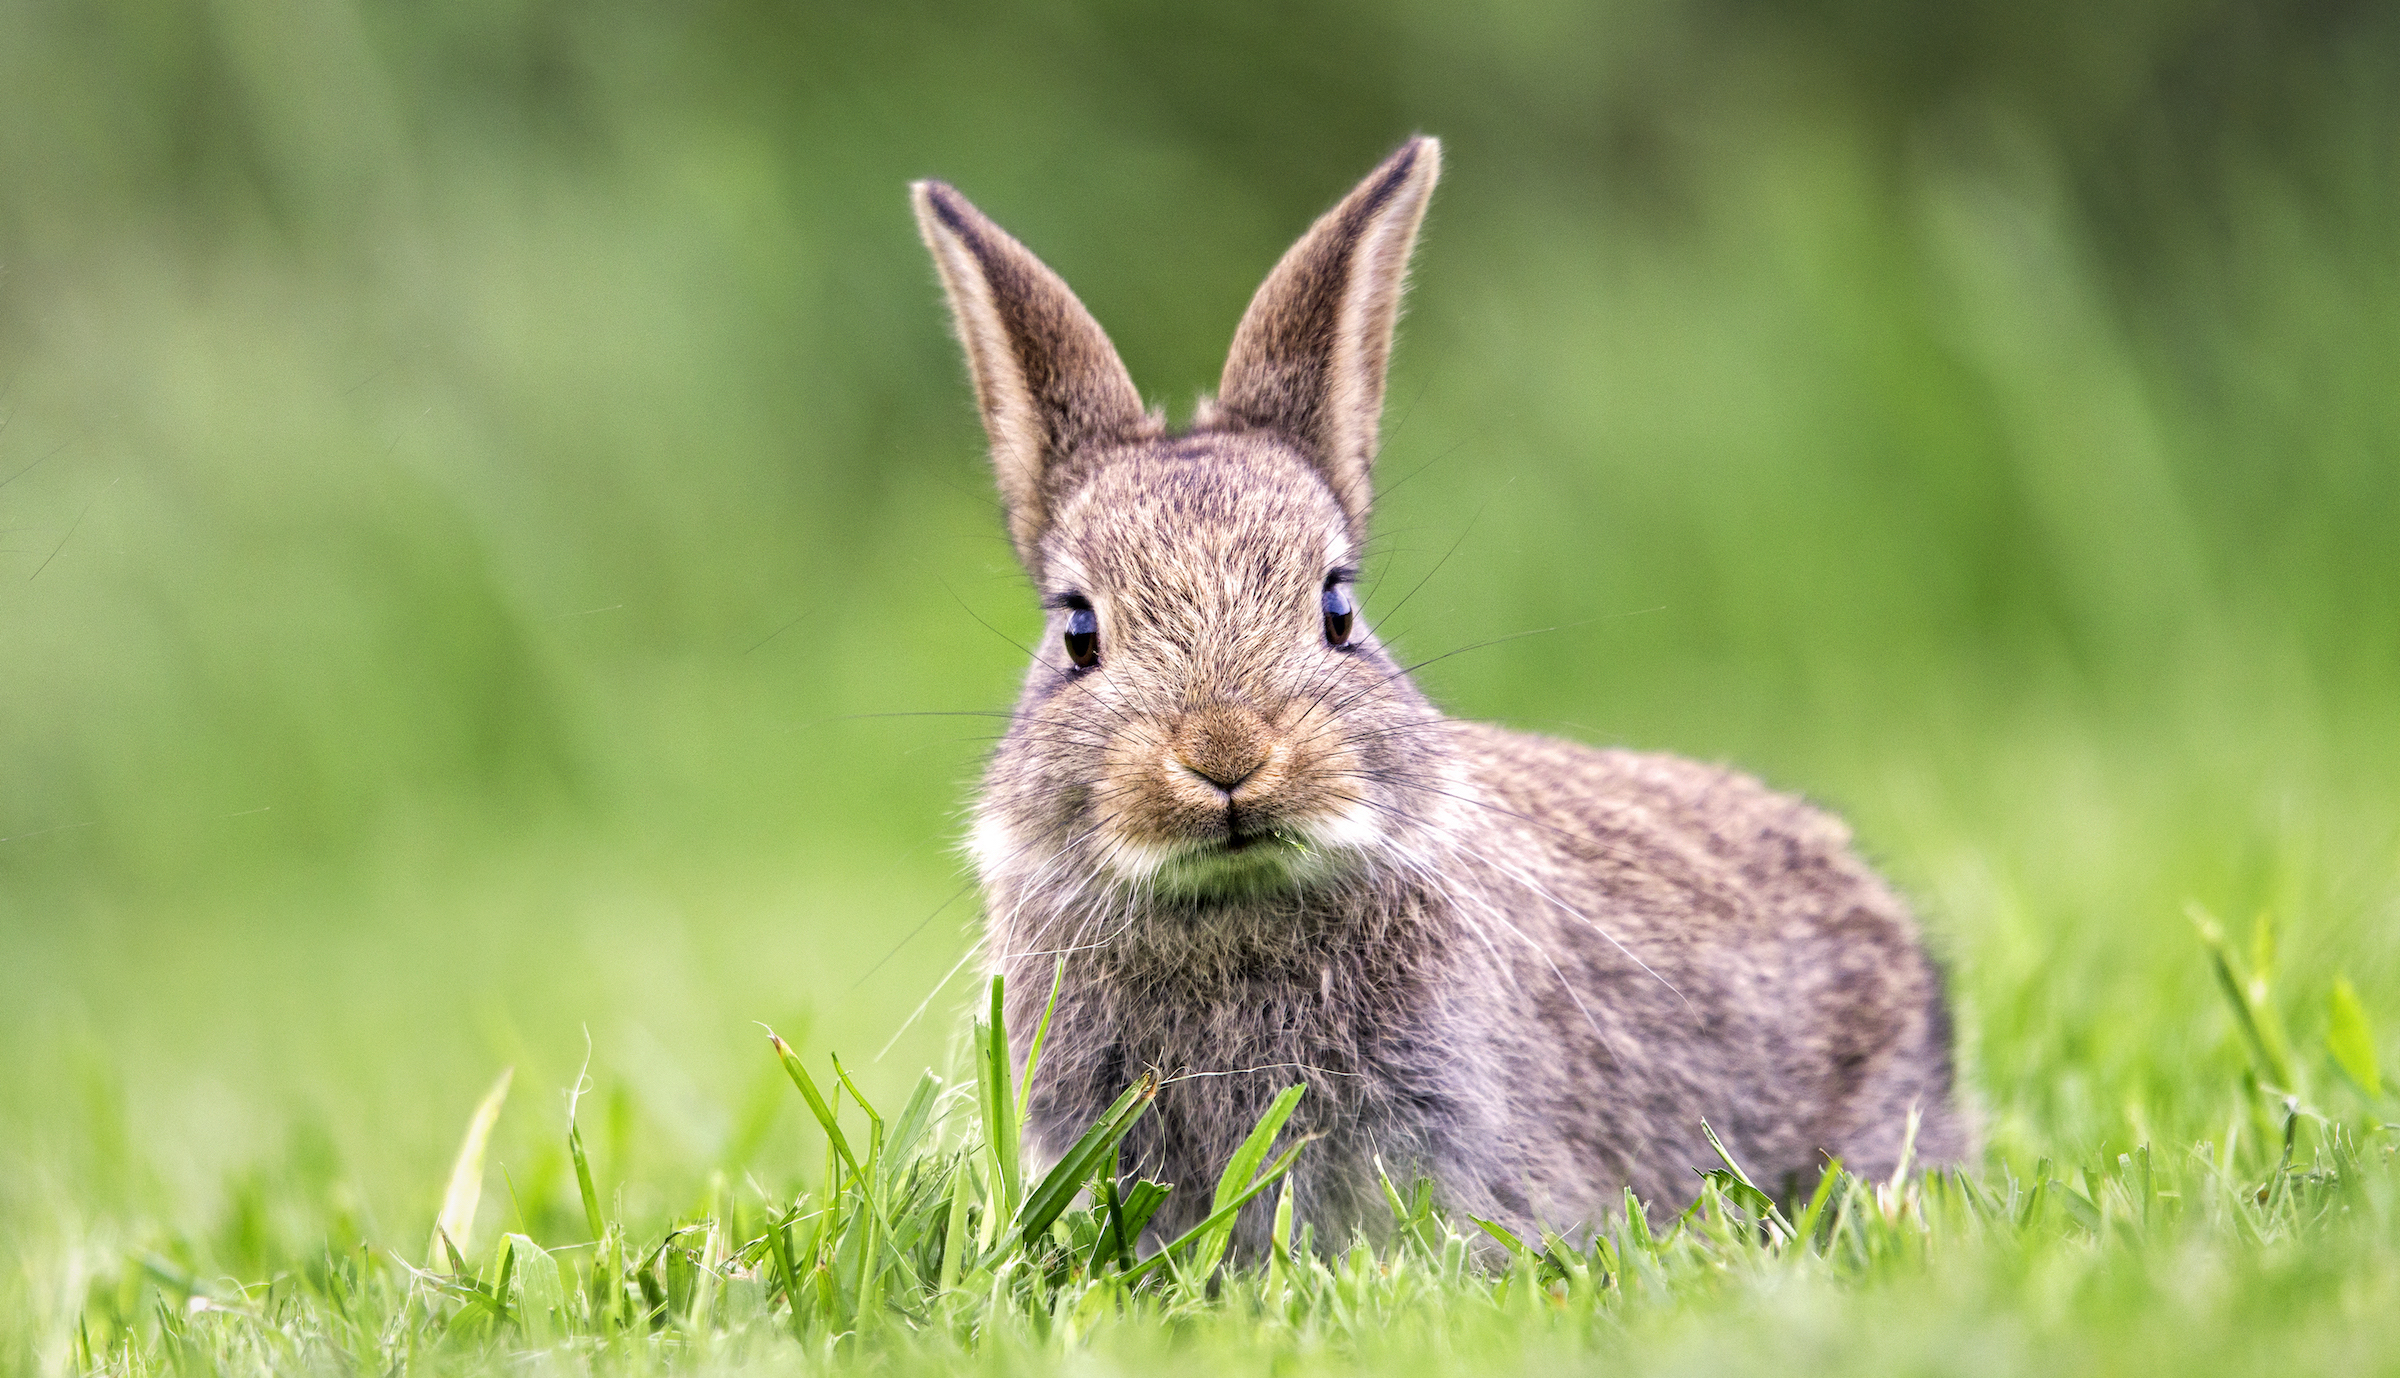
\includegraphics[scale=0.1]{rabbit}
\end{center}
\end{frame}

\begin{frame}
\begin{center}
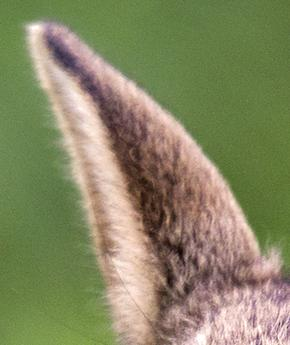
\includegraphics[scale=0.2]{ear1}\pause
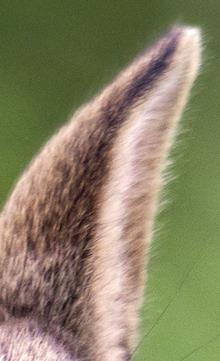
\includegraphics[scale=0.2]{ear2}\pause\\
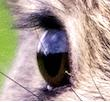
\includegraphics[scale=0.5]{eye1}\pause
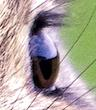
\includegraphics[scale=0.5]{eye2}\pause\\
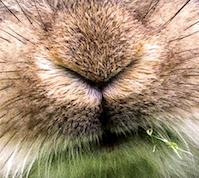
\includegraphics[scale=0.3]{nose}
\end{center}
\end{frame}


\begin{frame}
\begin{center}
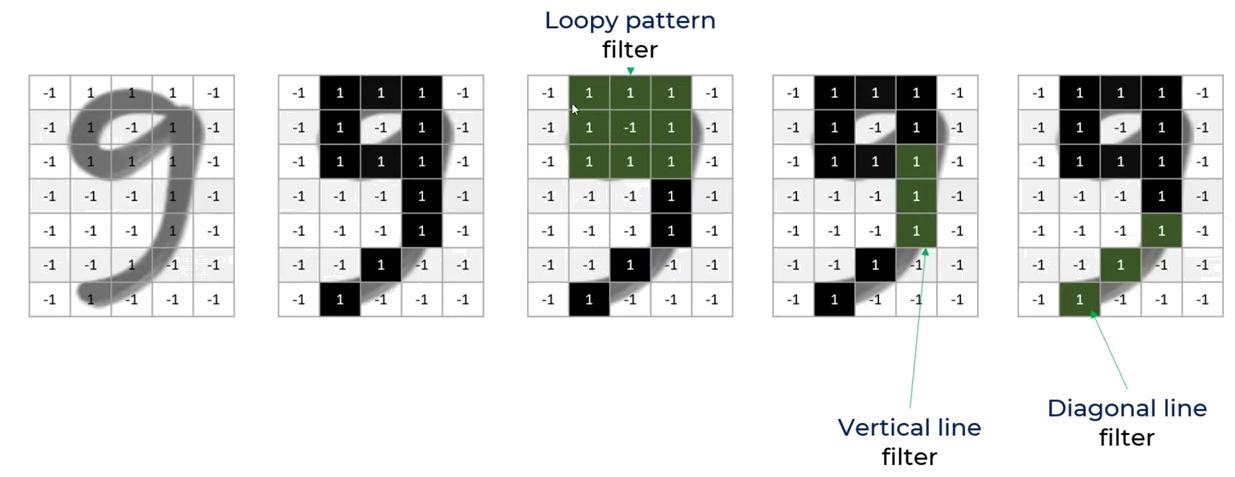
\includegraphics[scale=0.4]{nine}
\end{center}
\end{frame}


\begin{frame}
\begin{center}
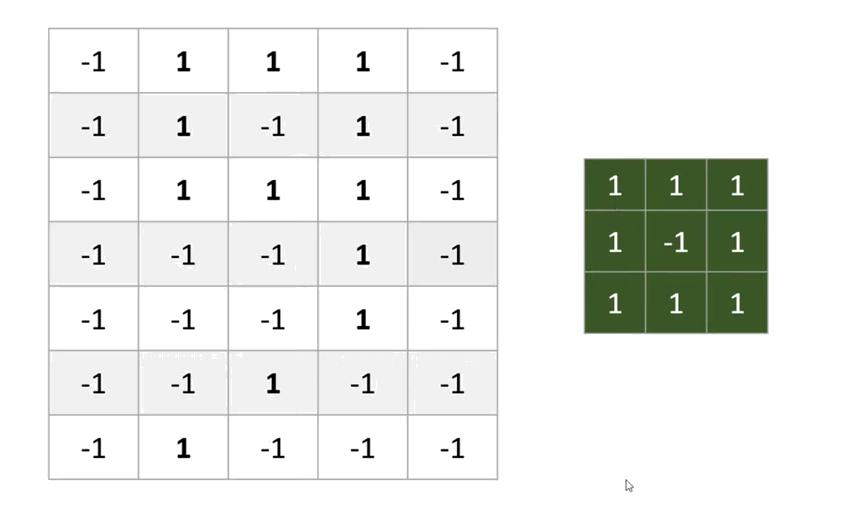
\includegraphics[scale=0.4]{nine2}
\end{center}
\end{frame}

\begin{frame}
\frametitle{Convolution}
\begin{itemize}
\item Let $x(t)$ be a noisy signal of a variable that depend on the time.
\smallskip
\item Let $w(t')$ be the weight function at time $t'$.
\smallskip
\item Then $s(t)=(x*w)(t)$ is the smoothed signal with respect to the weight $w$.
\[
s(t)=(x*w)(t)=\int_{-\infty}^{\infty}x(a)w(t-a)da
\]
\end{itemize}
\end{frame}

\begin{frame}
\begin{figure}
\begin{tikzpicture}
\node[red] at (0,0) {$x(t)$};
\node[red] at (0,1) {input};
\draw[->] (0.5,0) -- (2,0);
\draw[fill=pink] (2,-1) rectangle (4,1);
\draw[->] (4,0) -- (6,0);
\node[green] at (6.5,0) {$s(t)$};
\node[green] at (6.5,1) {output};
\node[blue] at (3,0) {$\_*w$};
\draw[->] (3,2) -- (3,1);
\node[blue] at (3,2.5) {$w$};
\node[blue] at (3,3) {kernel};
\end{tikzpicture}
\end{figure}
\end{frame}


\begin{frame}
\frametitle{Discerete Convolution}
\[
S(i,j)=(X*K)(i,j)=\sum_{m=-\infty}^{\infty}\sum_{n=-\infty}^{\infty}X(i-m,j-n)K(m,n)
\]
This operator has commutative property, i.e.,
\[
(X*K)(i,j)=(K*X)(i,j)
\]
\end{frame}

\begin{frame}
\frametitle{Cross-correlation}
\[
S(i,j)=(X*K)(i,j)=\sum_{m=-\infty}^{\infty}\sum_{n=-\infty}^{\infty}X(i+m,j+n)K(m,n)
\]
This operator does not have the commutative property, i.e.,
\[
(X*K)(i,j)\neq (K*X)(i,j)
\]
\end{frame}

\begin{frame}
\frametitle{Why Convolutional Networks}
\begin{itemize}
\item Sparse interactions.
\bigskip
\item Parameter sharing.
\bigskip
\item Equivalent representation.
\end{itemize}
\end{frame}

\begin{frame}
\begin{center}
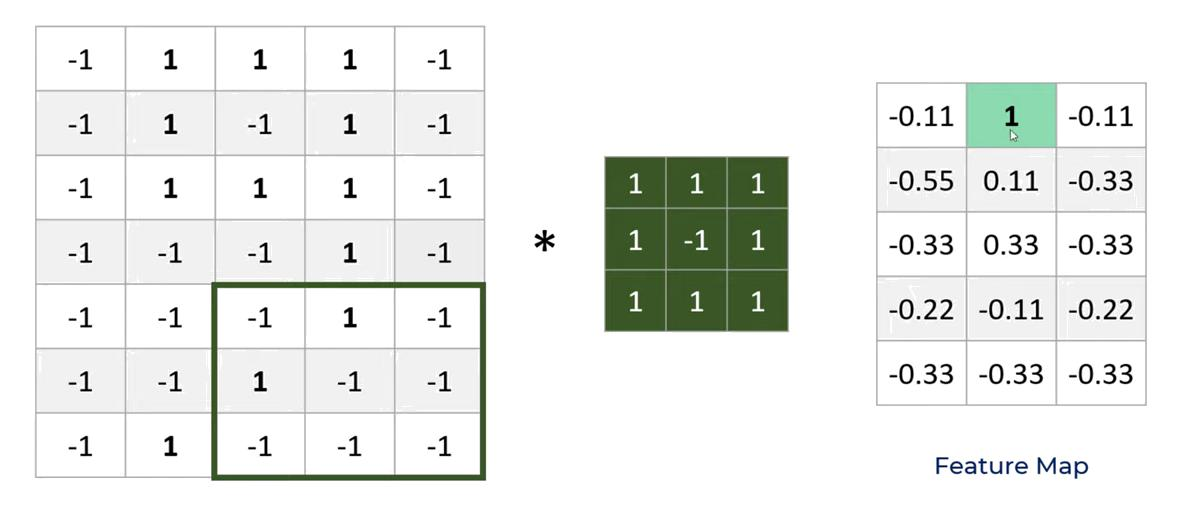
\includegraphics[scale=0.4]{nine3}
\end{center}
\end{frame}


\begin{frame}
\begin{center}
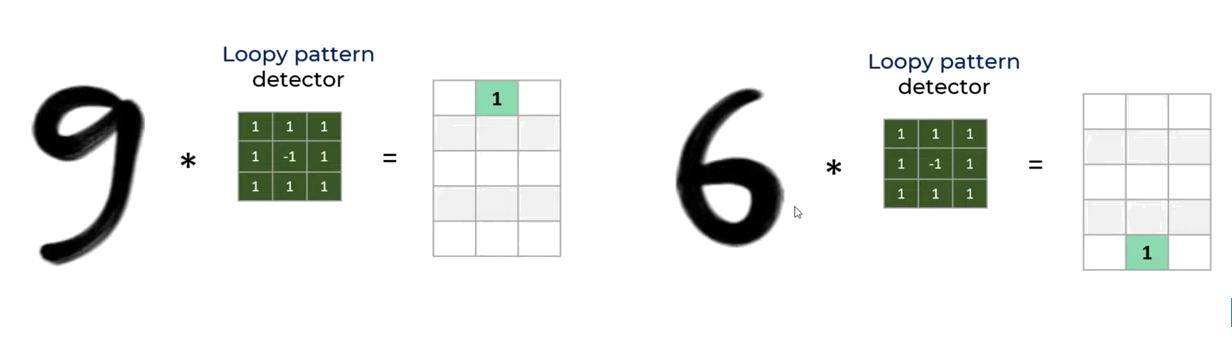
\includegraphics[scale=0.4]{nine4}
\end{center}
\end{frame}


\begin{frame}
\begin{center}
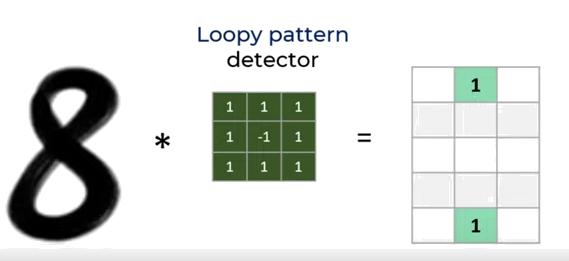
\includegraphics[scale=0.4]{eight}
\end{center}
\end{frame}


\begin{frame}
\begin{center}
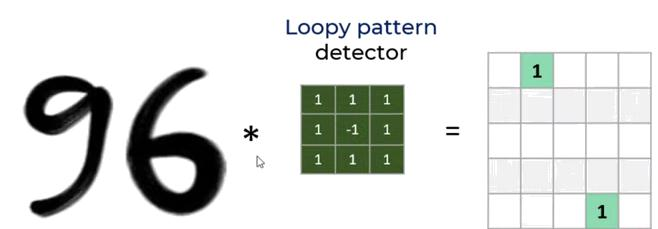
\includegraphics[scale=0.4]{ninesix}
\end{center}
\end{frame}

\begin{frame}
\begin{center}
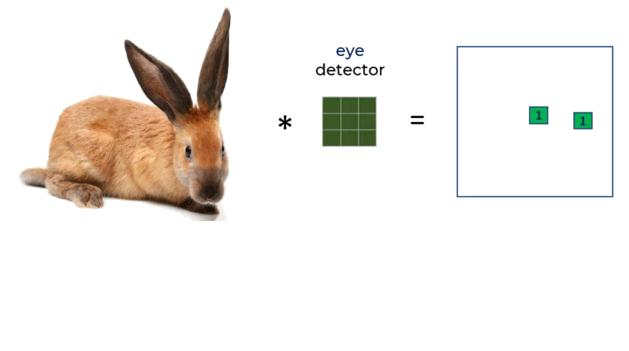
\includegraphics[scale=0.6]{eyedetect}
\end{center}
\end{frame}

\begin{frame}
\begin{center}
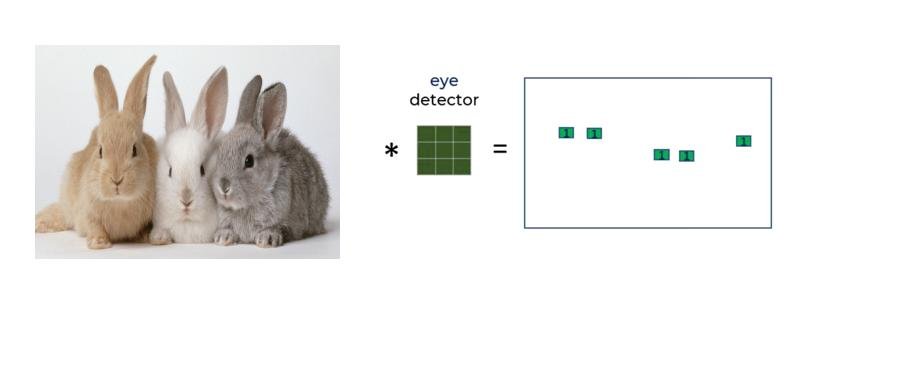
\includegraphics[scale=0.6]{eyedetect2}
\end{center}
\end{frame}

\begin{frame}
\frametitle{Pooling}
\begin{itemize}
\item A pooling function replaces the output of the net at a certain location with a summary statistic of the nearby output.
\bigskip
\item For creating a condensed feature map (reduce dimensionality).
\bigskip
\item The \textbf{max pool} report the maximum output within a rectangular neighborhood.
\end{itemize}
\end{frame}

\begin{frame}

\begin{center}
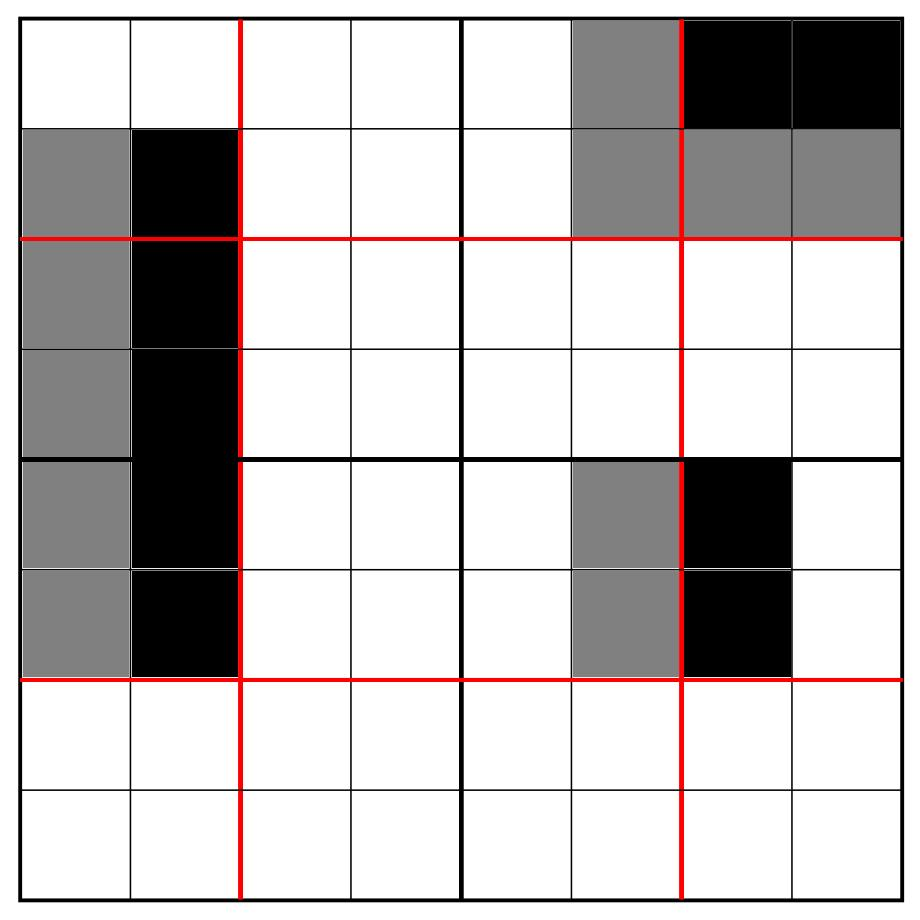
\includegraphics[scale=0.2]{pooling1}\pause \hspace{20pt} $\Longrightarrow$
\hspace{20pt} 
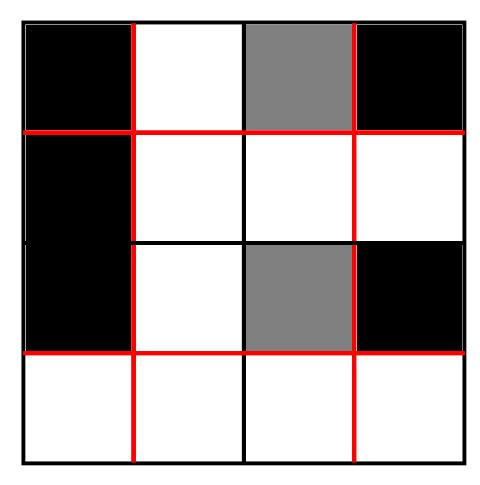
\includegraphics[scale=0.2]{pooling2}
\end{center}

\end{frame}

\begin{frame}
\frametitle{Padding}
\begin{itemize}
\item The shape of input image $X$ is $m\times n$.
\bigskip
\item The shape of kernel $K$ is $f\times f$.
\bigskip
\item Then the shape of output $S=X*K$ is $(m-f+1)\times (n-f+1)$.
\bigskip
\item So the output does not have the same shape as input.
\end{itemize}
\end{frame}

\begin{frame}
\begin{center}
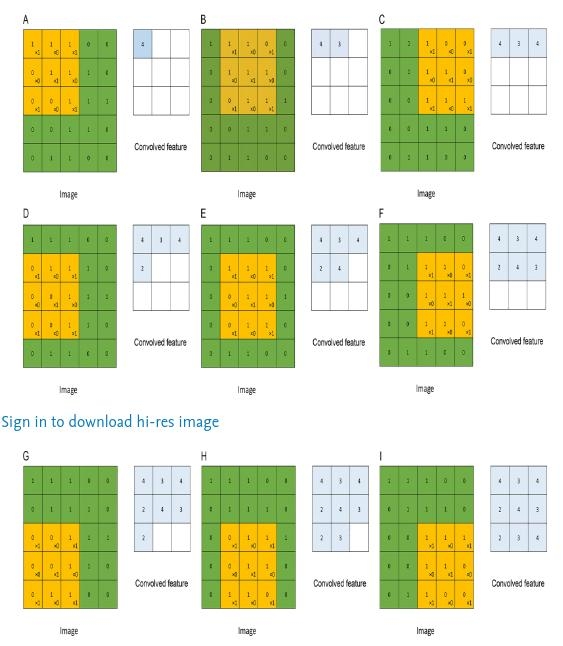
\includegraphics[scale=0.5]{padding2}
\end{center}
\end{frame}

\begin{frame}
\frametitle{Padding}
\begin{itemize}
\item The process of adding extra layers to the input image to avoid input/output shape difference is called \textbf{padding}.\pause
\begin{center}
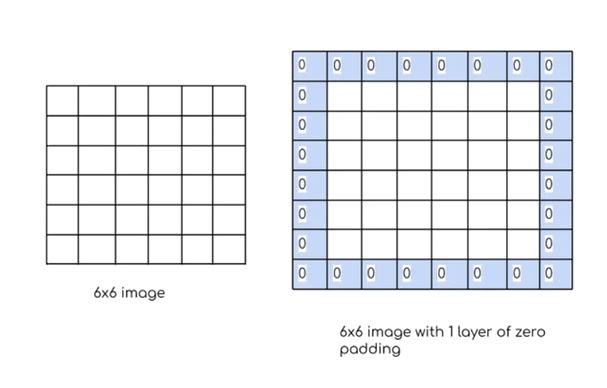
\includegraphics[scale=0.6]{padding}
\end{center}
\end{itemize}
\end{frame}

\begin{frame}
\frametitle{Types of Padding}
\begin{enumerate}
\item \textbf{Valid padding:} no padding, i.e.,
\[
\textbf{input: }m\times n \xrightarrow[]{\textbf{filter: } f\times f} \textbf{output: }(m-f+1)\times (n-f+1)
\]\pause
\item \textbf{Same padding:}output has the same shape as the input if we add $p$ layes of padding to the border. i.e.,\pause
\[
\textbf{input: }m\times n \xrightarrow[]{\textbf{padding: }p}\textbf{padded: }(m+2p)\times (n+2p) \xrightarrow[]{\textbf{filter: } f\times f} \textbf{output: }m\times n
\]\pause
for same padding $p$ should be equal to $\frac{f-1}{2}$.
\end{enumerate}
\end{frame}



\begin{frame}
\begin{center}
\begin{tikzpicture}
\draw[fill=pink] (0,0) rectangle (2,1);
\node[] at (1,0.5) {Input};
\draw[fill=blue!20] (-1.5,1) rectangle (3.5,7);
\node[] at (1,6) {Convolutional Layer};
\draw[fill=pink] (-1,2.5) rectangle (3,1.5);
\node[] at (1,2) {Convolutional Stage};
\draw[fill=pink] (-1,3) rectangle (3,4);
\node[] at (1,3.5) {Detector Stage};
\draw[fill=pink] (-1,4.5) rectangle (3,5.5);
\node[] at (1,5) {Pooling Stage};
\draw[fill=pink] (0,7) rectangle (2,8);
\node[] at (1,7.5) {Next Layer};
\draw[->] (1,1) -- (1,1.5);
\draw[->] (1,2.5) -- (1,3);
\draw[->] (1,4) -- (1,4.5);
\draw[->] (1,5.5) -- (1,7);

\end{tikzpicture}
\end{center}
\end{frame}

\begin{frame}{}
  \centering \Huge
  \emph{Thank You}
\end{frame}

\end{document}

